\documentclass[letterpaper]{article}
\title{16831 Statistical Techniques, Fall 2011\\Homework 5: Online Learning}
\date{December 7th, 2011}
\author{Natasha Kholgade and Marynel V\'azquez}
\usepackage[margin=1in]{geometry}
\usepackage{amsmath}
\usepackage{amssymb}
\usepackage{url}
\usepackage{graphicx}
\usepackage{color}
% Make URL click-able
\usepackage{hyperref}

% Don't indent after paragraphs
\parindent 0in
\parskip 4pt

\begin{document}

\maketitle

\section*{Classifiers}
For this homework, we implemented Gaussian Process Regression (GPR),
Adaptive Boosting, and online linear SVMs. We used these algorithms in a binary
fashion to classify 3D points into five different classes: Vegetation,
Wire, Pole, Ground and Facade. Each classifier was trained 5 times in
a one-vs-all scenario, such that the final classification for a
testing data point was given by the class with highest score.

GPR and boosting were not implemented in an online fashion (though
boosting does lend itself to an online implementation, we were limited
in time). Our version of Gaussian Process Regression uses the
exponential to the negative squared distance between features (radial
basis function) as the covariance function. Meanwhile, boosting
performs feature selection, and uses the exponentiated gradient as
suggested by Alex Grubb. We use thresholded decision stumps as linear
classifiers in boosting.

Our implementation of a linear Supper Vector Machine is based on the
subgradient of the hinge loss, plus a regularization term. We followed
Drew's notes, and used a learning rate equal to $\alpha = c/(\lambda(t
+ t_0))$. It operates fast, though requires a significant number of
samples to satisfactory classify new data in comparison to the other
algorithms being considered.

\section*{Performance Summary}
For this homework, we performed two-fold cross-validation on data from
one file, and then tested with data from the other file. We swapped
the two files, and re-did cross-validation and training. We provide
the best parameters, confusion matrices, per-class percentage
performance, and net classification rate for the three classes.

For brevity, we refer to the point cloud data file
\textit{oakland\_part3\_am\_rf.node\_features} as \textit{File\_am}, and
to the file \textit{oakland\_part3\_an\_rf.node\_features} as
\textit{File\_an} in the following sections.

\subsection*{Gaussian Process Regression}

\textbf{Train with \textit{File\_am}, and test with \textit{File\_an}:}

Best parameters: radial basis function parameter $\sigma=.4$,
regularization parameter $\lambda=.4642$.

Net classification rate: .$8637$.

Per-class classification rate: 
$$\begin{bmatrix}0.8208   & 0.8870  &  0.7192   & 0.9796 &   0.6670\end{bmatrix}$$

\textbf{Train with \textit{File\_an}, and test with \textit{File\_am}:}

Best parameters: radial basis function parameter $\sigma=.4$, regularization parameter $\lambda=.4642$.

Net classification rate: $.947$.

Per-class classification rate: 
$$\begin{bmatrix}0.8097  &  0.5697   & 0.9279   & 0.9899  &  0.8305\end{bmatrix}$$

\begin{figure}
\begin{minipage}{.45\linewidth}
   
\includegraphics[width=\linewidth]{confusionmatrices/gpr_train_am_test_an.png}
   \small\centerline{Test with File\_an}\normalsize
   \end{minipage}
\begin{minipage}{.45\linewidth}
   
\includegraphics[width=\linewidth]{confusionmatrices/gpr_train_an_test_am.png}
   \small\centerline{Test with File\_am}\normalsize
   \end{minipage}
   \caption{Confusion matrices for GPR classification.}
\end{figure}

\subsection*{Linear SVMs}

\textbf{Train with \textit{File\_am}, and test with \textit{File\_an}:}

Best parameters: For the learning rate $\alpha = c/(\lambda(t + t_0))$,
we found as best combination $\lambda = 10^{-4}$, $c = 1$, and $t_0 = 100$.

Net classification rate: $0.7462$

Per-class classification rate: 
\[
\begin{bmatrix} 0.5581 & 0.1549 & 0.3610 & 0.9988 & 0.9445\end{bmatrix}
\]

\textbf{Train with \textit{File\_an}, and test with \textit{File\_am}:}

Best parameters: For the learning rate $\alpha = c/(\lambda(t + t_0))$,
we found as best combination $\lambda = 10^{-4}$, $c = 1$, and $t_0 = 10$.

Net classification rate: $0.9567$

Per-class classification rate: 
\[
\begin{bmatrix}
0.8893    & 0.4450    & 0.6634    & 0.9941    & 0.8644
\end{bmatrix}
\]


\begin{figure}
\begin{minipage}{.45\linewidth}
   
\includegraphics[width=\linewidth]{confusionmatrices/confusionSVMQ1_1.png}
   \small\centerline{Test with File\_an}\normalsize
   \end{minipage}
\begin{minipage}{.45\linewidth}
   
\includegraphics[width=\linewidth]{confusionmatrices/confusionSVMQ1_2.png}
   \small\centerline{Test with File\_am}\normalsize
   \end{minipage}
   \caption{Confusion matrices for linear SVM classification.}
\end{figure}


\subsection*{AdaBoost}
\textbf{Train with \textit{File\_am}, and test with \textit{File\_an}:}

Best parameters: Running time $T=140$, gradient projection threshold $\eta=1e-4$.

Net classification rate: $.8663$.

Per-class classification rate: 
$$\begin{bmatrix} 0.8403  &  0.8560   & 0.7017 &   0.9798  &  0.6476\end{bmatrix}$$

\textbf{Train with \textit{File\_an}, and test with \textit{File\_am}:}

Best parameters: Running time $T=140$, gradient projection threshold $\eta=1e-4$.

Net classification rate: $.9495$.

Per-class classification rate: 
$$\begin{bmatrix}0.8178 &   0.6320 &   0.9104  &  0.9948  &  0.8148\end{bmatrix}$$
\begin{figure}
\begin{minipage}{.45\linewidth}
   
\includegraphics[width=\linewidth]{confusionmatrices/boost_train_am_test_an.png}
   \small\centerline{Test with File-an}\normalsize
   \end{minipage}
\begin{minipage}{.45\linewidth}
   
\includegraphics[width=\linewidth]{confusionmatrices/boost_train_an_test_am.png}
   \small\centerline{Test with File-am}\normalsize
   \end{minipage}
   \caption{Confusion matrices for classification with AdaBoost.}
\end{figure}

\subsection*{Time}
AdaBoost takes on average a long time to train (148 seconds) but just
1.12 seconds in testing as we just apply a set of thresholded linear
classifiers and take their sum. 

GPR takes lesser training time (12.19
seconds), but it takes a longer test time (26.83 seconds), because we
apply the product of the training kernel matrix inverse and the
training labels (which can be precomputed) to all the kernel vectors
formed with every test point to all training points.

SVM took even less training time (5.46 seconds in average) and testing
time (0.03 seconds). Training took longer than testing given that 5
classifiers were built in total.  Testing only required to find
out which of these classifiers gave the best score.

\subsection*{Misclassifications}
We find that points belonging to the `Pole', `Wire', and `Facade'
classes do not always perform well. Our intuition was that there is
not enough data to learn these classes well, so for GPR and Adaboost
we subsampled the data provided to create a training set with similar
number of examples per class. Given an initial set of training data,
we looked for the class with less number of examples (N), and then
randomly selected N data points from the other classes. We finally
trained using 5N data points.

We also tested the subsampling strategy with our online SVM, but
couldn't find any classification improvement. Thus, the results
presented in this report are those generated using all the available
training data.

\subsection*{Ease of Implementation}
GPR and SVM were relatively easy to implement. AdaBoost required a bit of delving into some math, but we made it through.
\subsection*{Robustness to noise}
GPR is robust to noise. When we added a whole bunch of noise to the features, we still get net classification rates of .865 and .94, and per-class correct classifications:
$$\begin{bmatrix} 0.8417 &   0.8614 &   0.7164   & 0.9806  &  0.6263\end{bmatrix}$$
$$\begin{bmatrix} 0.7809  &  0.5733  &  0.9440&    0.9969    &0.7608\end{bmatrix}$$
Noise-corrupted versions of features when passed through GPR are classified with rates .85 and .94, and per-class classifications are:
$$\begin{bmatrix} 0.8204  &  0.8757 &   0.6980  &  0.9796 &   0.5859\end{bmatrix}$$
$$\begin{bmatrix} 0.7779  &  0.5880  &  0.9286  &  0.9950 &   0.7704\end{bmatrix}$$

The same robustness is observed with AdaBoost. On adding a whole bunch of noise to the features, we get rates of .862, and .947, and per-class classifications of:
$$\begin{bmatrix} 0.8334 &   0.8514 &   0.6796  & 0.9775  &  0.6465\end{bmatrix}$$
$$\begin{bmatrix} 0.7985 &   0.6064   & 0.9146 &   0.9935 &   0.8167\end{bmatrix}$$
Noise-corrupted versions of features when passed through AdaBoost are classified with rates .8676 and .945, and per-class classifications are:
$$\begin{bmatrix} 0.8543 &   0.8548 &   0.6888&    0.9725  &  0.6410\end{bmatrix}$$
$$\begin{bmatrix} 0.8063  &  0.6112 &   0.9174  &  0.9918  &  0.8062\end{bmatrix}$$

Likewise, we observed for the SVM that adding random noise to the
features did not impact performance negatively. We get rates of 0.767
and 0.958, with per-class classifications as follows:
$$\begin{bmatrix} 0.5970    & 0.1951    & 0.4521    & 0.9984   & 0.9456\end{bmatrix}$$
$$\begin{bmatrix} 0.8776  &  0.4474  &  0.7047  &  0.9975  &  0.8608\end{bmatrix}$$

The results for the SVM were very interesting when we input
noise-corrupted features, as we obtained 0.806 and 0.9519. We believe
that the noise in this case led to learn a classifier that could
generalize better, by reducing the chances of overfitting. The
per-class classification results were:
$$\begin{bmatrix} 0.6839  &  0.4667  &  0.2928  &  0.9991  &  0.8873\end{bmatrix}$$
$$\begin{bmatrix} 0.9189   & 0.4511   & 0.6060    & 0.9941   & 0.8153\end{bmatrix}$$

\subsection*{Final Remarks}

We would most probably use AdaBoost for the robot because it is faster
than Gaussian Process Regression during testing (though it performs
just as well), and it performs better than the linear SVM. If we
needed an online version of the training algorithm, we would probably
use SVMs, but with kernels. We did not have time to implement the
kernel SVMs, but we do notice that the dataset has some non-linearity
as is evidenced by the better performance of GPR and AdaBoost.

\subsection*{Pictorial Result}
With GPR training with \textit{File\_am}, and testing with \textit{File\_an} gave us the scatter plot shown in \ref{Fig_GPR1}, while training with \textit{File\_an}, and testing with \textit{File\_am} gave us the plot in \ref{Fig_GPR2}
\begin{figure}
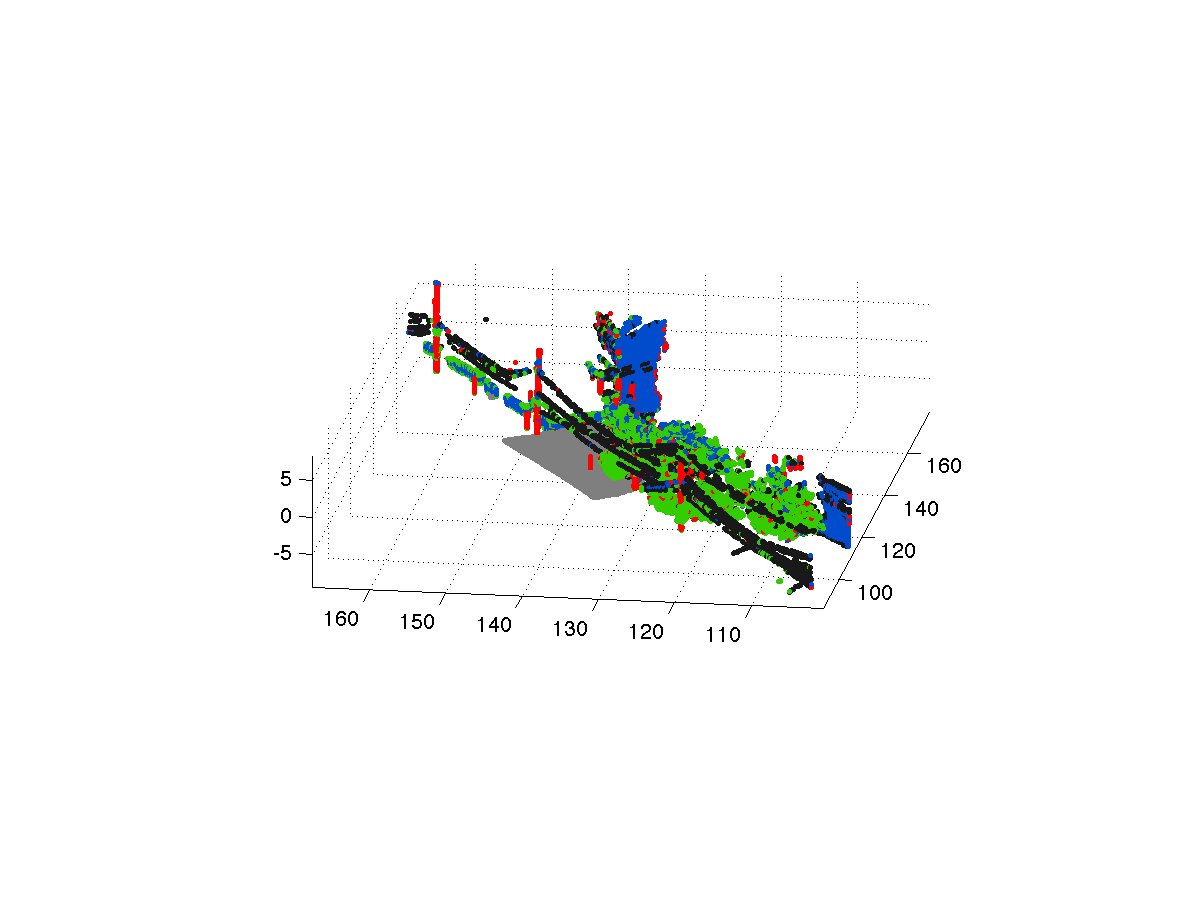
\includegraphics[width=.8\linewidth]{gpr_trainam_testan.png}
\caption{Scatter plot of points from File-am classified with GPR: green = vegetation, blue = facade, really dark gray = wire, red = pole, light gray = ground}
\label{Fig_GPR1}
\end{figure}
\begin{figure}
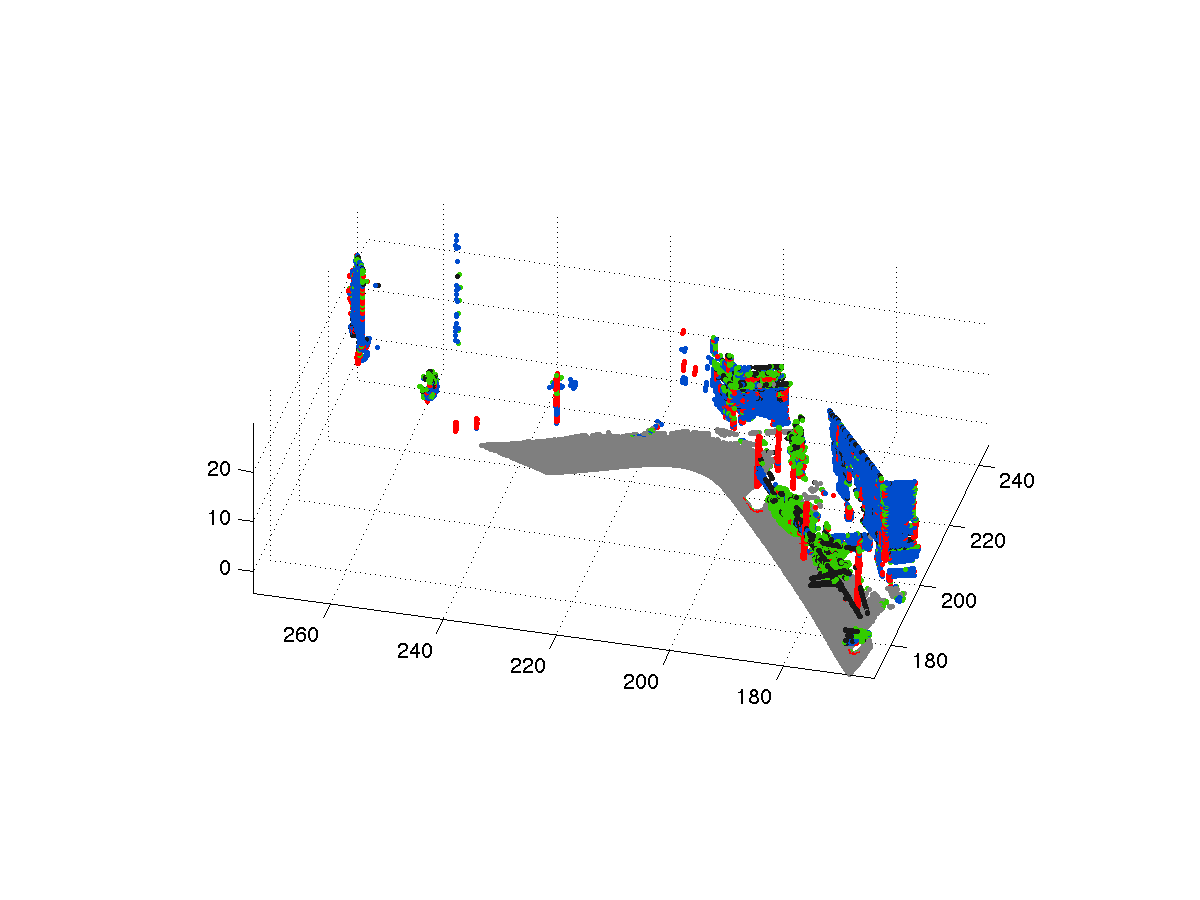
\includegraphics[width=.8\linewidth]{gpr_trainan_testam.png}
\caption{Scatter plot of points from File-an classified with GPR: green = vegetation, blue = facade, really dark gray = wire, red = pole, light gray = ground}
\label{Fig_GPR2}
\end{figure}

With AdaBoost training with \textit{File\_am}, and testing with \textit{File\_an} gave us the scatter plot shown in \ref{Fig_Ada1}, while training with \textit{File\_an}, and testing with \textit{File\_am} gave us the plot in \ref{Fig_Ada2}
\begin{figure}[t]
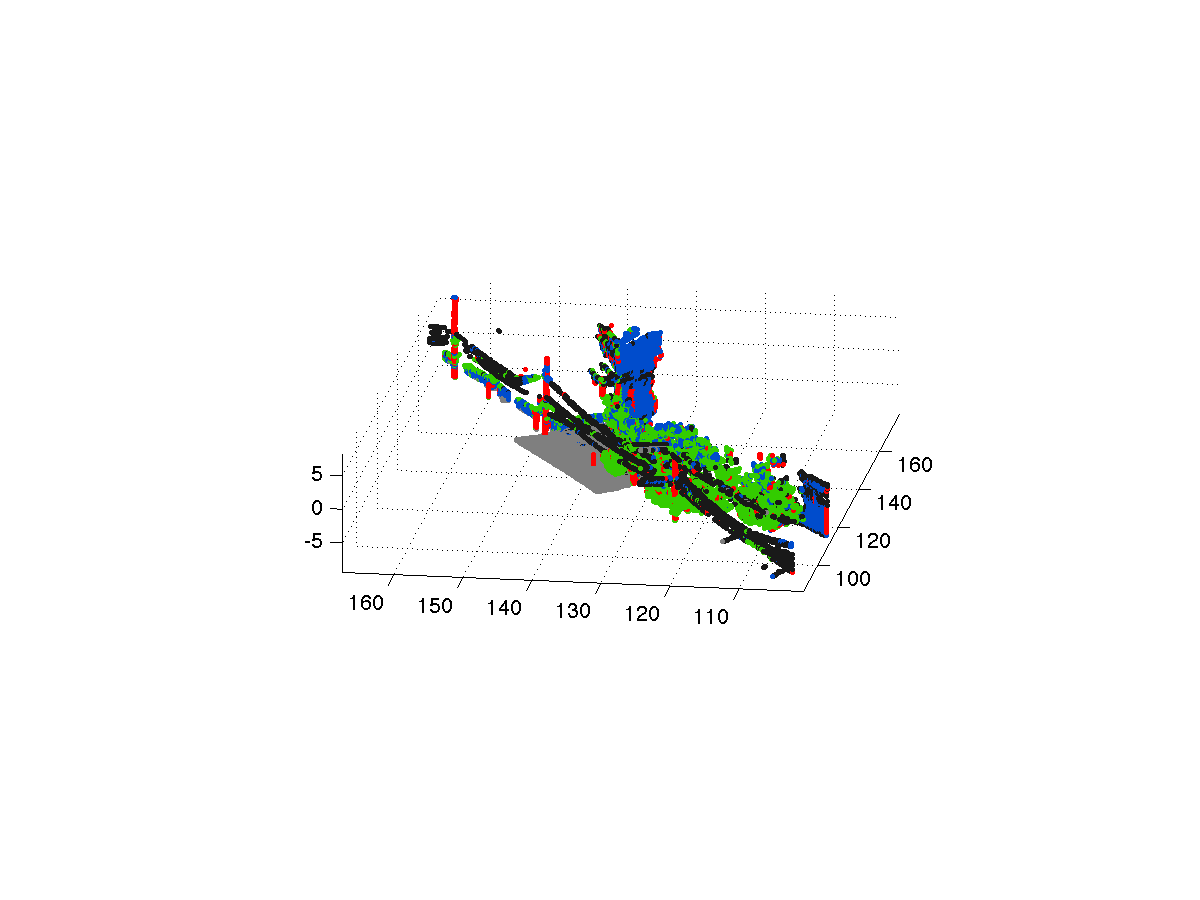
\includegraphics[width=.8\linewidth]{boost_trainam_testan.png}
\caption{Scatter plot of points from File-am classified with AdaBoost: green = vegetation, blue = facade, really dark gray = wire, red = pole, light gray = ground}
\label{Fig_Ada1}
\end{figure}
\begin{figure}[t]
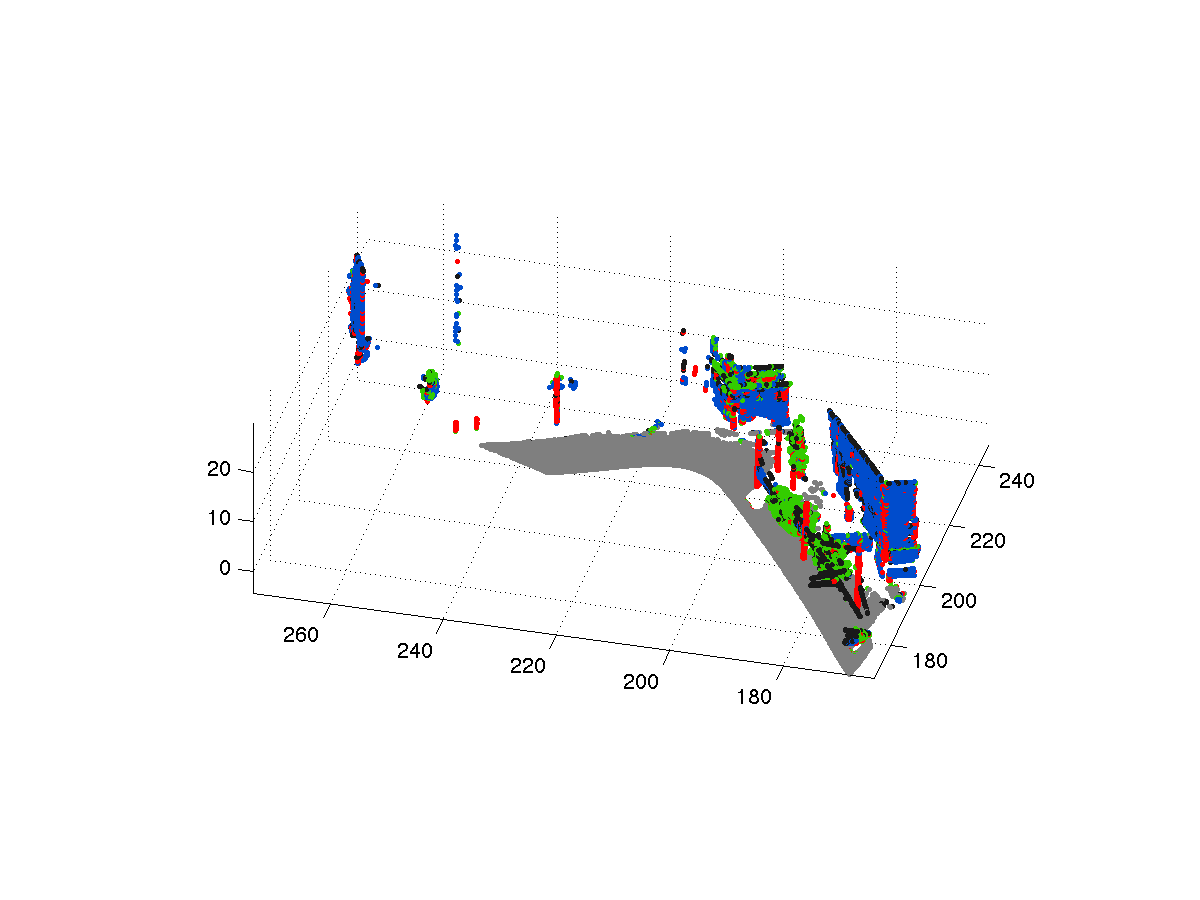
\includegraphics[width=.8\linewidth]{boost_trainan_testam.png}
\caption{Scatter plot of points from File-an classified with AdaBoost: green = vegetation, blue = facade, really dark gray = wire, red = pole, light gray = ground}
\label{Fig_Ada2}
\end{figure}


\begin{enumerate}
\item How well did it perform for online learning?  Does it perform well on the held-out data?
\item Are there any classes that did not get classified well?  Why do you think that is?
\item How easy was the learner to implement?
\item How long does the learner take (in terms of data points, dimensions, classes, etc...) for training and prediction?
\item Show images/movies of the classified data.  Note that MATLAB is not very good at displaying thousands of 3D points; use VRML or python.
\item How did you choose (hyper)parameters (priors, kernel width, noise variance, prior variance, learning rate, etc\ldots)?
\item How robust is this algorithm to noise? Take the current feature set and:
  \begin{itemize}
  \item Add a large number of random features
  \item Add a large number of features that are noise corrupted versions of the features already in the data-set.
  \end{itemize}

\end{enumerate}

You should also compare the learners' performance to each other.  Did kernels help on this data set?  Which one would you use on your robot?  What would future work include?

\end{document}
